\documentclass[12pt,a4paper]{article}

% ─── Page Layout ───────────────────────────────────────────────────────────────
\usepackage[a4paper, margin=0.8in, headheight=14pt]{geometry}

% ─── Fonts (XeLaTeX) ───────────────────────────────────────────────────────────
\usepackage{fontspec}
\usepackage{unicode-math}
\setmainfont{TeX Gyre Pagella}
\setmonofont[Scale=0.88]{TeX Gyre Cursor}
\setmathfont{Latin Modern Math}

% ─── Packages ──────────────────────────────────────────────────────────────────
\usepackage{xcolor}
\usepackage{colortbl}
\usepackage{titlesec}
\usepackage{enumitem}
\usepackage{tabularx}
\usepackage{booktabs}
\usepackage{array}
\usepackage{amsmath}
\usepackage{tikz}
\usetikzlibrary{shapes.geometric, arrows.meta, positioning, calc, fit, decorations.pathreplacing, patterns}
\usepackage[american]{circuitikz}
\usepackage{tcolorbox}
\tcbuselibrary{skins, breakable}
\usepackage{hyperref}
\usepackage{fancyhdr}
\usepackage{graphicx}
\usepackage{microtype}
\hyphenpenalty=10000
\exhyphenpenalty=10000
\sloppy
\usepackage{caption}
\usepackage{setspace}
\usepackage{multirow}
\usepackage{tocloft}

% ─── Q&A helper ────────────────────────────────────────────────────────────────
\newcommand{\Q}[1]{\textbf{#1}\par\noindent\ignorespaces}

% ─── Colour Palette ────────────────────────────────────────────────────────────
\definecolor{myred}{RGB}{196,30,58}
\definecolor{mydark}{RGB}{30,30,50}
\definecolor{mygreen}{RGB}{14,120,80}
\definecolor{myteal}{RGB}{0,130,140}
\definecolor{myamber}{RGB}{180,100,0}
\definecolor{mypurple}{RGB}{100,30,160}
\definecolor{mygray}{RGB}{246,247,249}
\definecolor{mgframe}{RGB}{180,185,200}
\definecolor{watermark}{RGB}{145,150,170}
\definecolor{hdrred}{RGB}{250,232,235}
\definecolor{hdrgreen}{RGB}{220,244,233}
\definecolor{hdrteal}{RGB}{220,242,244}
\definecolor{hdramber}{RGB}{253,242,215}
\definecolor{hdrpurple}{RGB}{238,228,255}
\definecolor{hdrgray}{RGB}{238,240,245}
\definecolor{rowalt}{RGB}{250,251,253}

% ─── Section Formatting ────────────────────────────────────────────────────────
\titleformat{\section}{\large\bfseries\color{myred}}{\thesection.}{0.5em}{}[\vspace{1pt}{\color{myred}\rule{\linewidth}{0.8pt}}]
\titleformat{\subsection}{\normalsize\bfseries\color{myteal}}{\thesubsection}{0.5em}{}
\titlespacing*{\section}{0pt}{18pt}{7pt}
\titlespacing*{\subsection}{0pt}{11pt}{4pt}

% ─── Paragraph ─────────────────────────────────────────────────────────────────
\setlength{\parindent}{0pt}
\setlength{\parskip}{4pt}

% ─── TOC Styling ───────────────────────────────────────────────────────────────
\renewcommand{\cfttoctitlefont}{\large\bfseries\color{myred}}
\renewcommand{\cftaftertoctitle}{\par\noindent{\color{myred}\rule{\linewidth}{0.8pt}}}
\setlength{\cftbeforetoctitleskip}{0pt}
\setlength{\cftaftertoctitleskip}{6pt}
\renewcommand{\cftsecfont}{\normalsize\bfseries\color{mydark}}
\renewcommand{\cftsecpagefont}{\normalsize\bfseries\color{mydark}}
\renewcommand{\cftsecleader}{\cftdotfill{\cftdotsep}}
\setlength{\cftbeforesecskip}{7pt}
\renewcommand{\cftsubsecfont}{\small\color{mydark}}
\renewcommand{\cftsubsecpagefont}{\small\color{mydark}}
\setlength{\cftbeforesubsecskip}{3pt}
\setlength{\cftsubsecindent}{1.4em}

% ─── Table helpers ─────────────────────────────────────────────────────────────
\renewcommand{\arraystretch}{1.45}
\setlength{\tabcolsep}{6pt}
\arrayrulecolor{mydark}
\newcolumntype{B}[1]{>{\small\bfseries\raggedright\arraybackslash}m{#1}}
\newcolumntype{Y}{>{\small\raggedright\arraybackslash}X}
\renewcommand{\tabularxcolumn}[1]{m{#1}}

% ─── Header / Footer ───────────────────────────────────────────────────────────
\pagestyle{fancy}
\fancyhf{}
\fancyhead[L]{\small\color{myred}\textbf{PE-EC802B}\;\color{mydark}--- Industrial Automation and Control}
\fancyhead[R]{\small\color{myteal}\textbf{Module 1 Notes}}
\fancyfoot[C]{\small\color{mydark}\thepage}
\fancyfoot[R]{\small\color{watermark}\textit{\copyright\ Biraj}}
\renewcommand{\headrulewidth}{0.5pt}
\renewcommand{\footrulewidth}{0.3pt}

% ─── Hyperref ──────────────────────────────────────────────────────────────────
\hypersetup{colorlinks=true, linkcolor=myteal, urlcolor=myteal,
  pdfauthor={Biraj Sarkar}, pdftitle={PE-EC802B --- Module 1 Notes}}

% ─── tcolorbox styles ──────────────────────────────────────────────────────────
\tcbset{
  tikzbox/.style={colback=mygray, colframe=mgframe, boxrule=0.6pt, arc=4pt,
    left=8pt, right=8pt, top=6pt, bottom=6pt,
    colbacktitle=mgframe, coltitle=mydark, fonttitle=\small\bfseries},
  defbox/.style={colback=hdrgreen, colframe=mygreen, boxrule=0.8pt, arc=4pt,
    left=9pt, right=9pt, top=6pt, bottom=6pt,
    colbacktitle=mygreen, coltitle=white, fonttitle=\small\bfseries},
  formulabox/.style={colback=hdrteal, colframe=myteal, boxrule=0.8pt, arc=4pt,
    left=9pt, right=9pt, top=7pt, bottom=7pt,
    colbacktitle=myteal, coltitle=white, fonttitle=\small\bfseries},
  examplebox/.style={colback=hdramber, colframe=myamber, boxrule=0.8pt, arc=4pt,
    left=9pt, right=9pt, top=6pt, bottom=6pt,
    colbacktitle=myamber, coltitle=white, fonttitle=\small\bfseries},
  masonbox/.style={colback=hdrpurple, colframe=mypurple, boxrule=0.8pt, arc=4pt,
    left=9pt, right=9pt, top=6pt, bottom=6pt,
    colbacktitle=mypurple, coltitle=white, fonttitle=\small\bfseries},
  exambox/.style={colback=hdrpurple, colframe=mypurple, boxrule=1pt, arc=5pt,
    left=10pt, right=10pt, top=8pt, bottom=8pt,
    colbacktitle=mypurple, coltitle=white, fonttitle=\bfseries,
    breakable, title after break={\textbf{Frequently Asked / Viva Questions (contd.)}}}
}
\tcbset{breakable}

% ─── TikZ styles ───────────────────────────────────────────────────────────────
\tikzset{
  block/.style={rectangle, draw=myteal, fill=hdrteal,
    text width=2.4cm, align=center, minimum height=0.95cm,
    font=\small, rounded corners=3pt, line width=0.7pt},
  redblock/.style={rectangle, draw=myred, fill=hdrred,
    text width=2.4cm, align=center, minimum height=0.95cm,
    font=\small, rounded corners=3pt, line width=0.7pt},
  sumjunc/.style={circle, draw=myamber, fill=hdramber,
    minimum size=0.62cm, font=\small, line width=0.8pt},
  arrow/.style={-Stealth, thick, color=mydark},
  line/.style={thick, color=mydark}
}

% ═══════════════════════════════════════════════════════════════════════════════
\begin{document}
% ═══════════════════════════════════════════════════════════════════════════════

\begin{center}
  {\LARGE\bfseries\color{myred} PE-EC802B --- Industrial Automation and Control}\\[5pt]
  {\normalsize\color{mydark} Semester VIII \quad$\bullet$\quad 3L:0T:0P \quad$\bullet$\quad 3 Credits}\\[3pt]
  {\normalsize\color{myteal}\textbf{Module 1 Exam Notes}}\\[3pt]
  {\small\color{mydark} CGEC \;$|$\; B.Tech ECE (2023--27) \;$|$\; \textit{Biraj Sarkar}}
\end{center}
\vspace{2pt}
\noindent{\color{myred}\rule{\linewidth}{1.5pt}}
\vspace{2pt}

\hypersetup{linkcolor=mydark}
\tableofcontents
\hypersetup{linkcolor=myteal}
\newpage

% ===============================================================================
\section{Introduction to Industrial Sensors and Actuators}
% ===============================================================================

In an industrial automation loop, \textbf{sensors} act as the "eyes" of the system by measuring physical process variables (temperature, pressure, flow) and converting them into electrical signals. \textbf{Actuators} act as the "hands" by executing the controller's decision (steering valves, turning motors, extending cylinders) to manipulate the physical process.

\begin{tcolorbox}[tikzbox, title={Standard Industrial Closed-Loop Control System}]
\centering
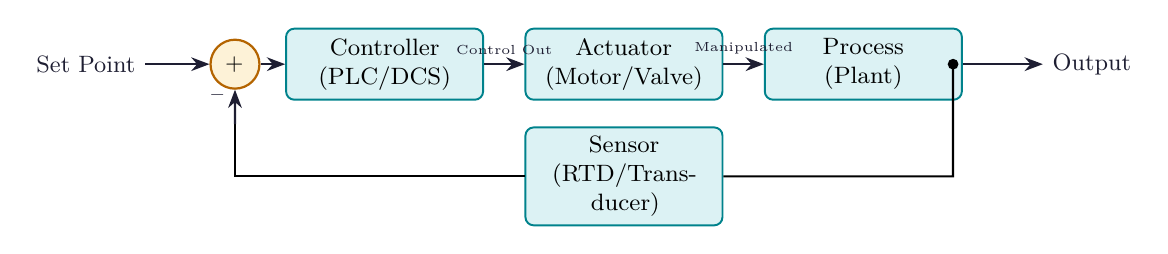
\begin{tikzpicture}[scale=0.95, transform shape]
  \node[block] (ctrl) at (0,0) {Controller\\(PLC/DCS)};
  \node[block] (act) at (3.2,0) {Actuator\\(Motor/Valve)};
  \node[block] (proc) at (6.4,0) {Process\\(Plant)};
  \node[block] (sens) at (3.2,-1.5) {Sensor\\(RTD/Transducer)};
  \node[sumjunc] (sum) at (-2.0,0) {$+$};

  % Paths
  \draw[arrow] (-3.2, 0) node[left, font=\small] {Set Point} -- (sum);
  \draw[arrow] (sum) -- (ctrl);
  \draw[arrow] (ctrl) -- (act) node[midway, above, font=\tiny] {Control Out};
  \draw[arrow] (act) -- (proc) node[midway, above, font=\tiny] {Manipulated};
  \draw[arrow] (proc) -- (8.8, 0) node[right, font=\small] {Output};
  
  \draw[thick] (7.6,0) to[short, *-] (7.6,-1.5) -- (sens);
  \draw[thick] (sens) -| (-2.0,-0.8);
  \draw[arrow] (-2.0,-0.8) -- (sum) node[left, pos=0.8, font=\scriptsize] {$-$};
\end{tikzpicture}
\end{tcolorbox}

% ===============================================================================
\section{Industrial Displacement and Force Sensors}
% ===============================================================================

\subsection{1. Linear Variable Differential Transformer (LVDT)}
An \textbf{LVDT} is an inductive, passive transducer that converts linear displacement into a proportional AC voltage.
\begin{itemize}[leftmargin=*, itemsep=2pt]
  \item \textbf{Structure:} Consists of a single primary winding ($P$) and two identical secondary windings ($S_1$ and $S_2$) wound symmetrically on a hollow cylindrical coil form, with a highly permeable nickel-iron magnetic core sliding inside.
\end{itemize}

\begin{tcolorbox}[tikzbox, title={LVDT Block Structure and Coil Connections}]
\centering
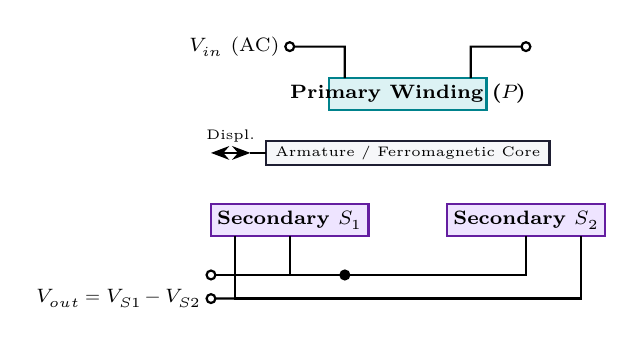
\begin{tikzpicture}[scale=1.0]
  % Primary coil
  \draw[thick, fill=hdrteal, draw=myteal] (-1.0, 0.6) rectangle (1.0, 1.0);
  \node[font=\scriptsize\bfseries] at (0, 0.8) {Primary Winding ($P$)};
  
  % Secondary coil 1
  \draw[thick, fill=hdrpurple, draw=mypurple] (-2.5, -0.6) rectangle (-0.5, -1.0);
  \node[font=\scriptsize\bfseries] at (-1.5, -0.8) {Secondary $S_1$};
  
  % Secondary coil 2
  \draw[thick, fill=hdrpurple, draw=mypurple] (0.5, -0.6) rectangle (2.5, -1.0);
  \node[font=\scriptsize\bfseries] at (1.5, -0.8) {Secondary $S_2$};
  
  % Core shaft
  \draw[thick, fill=mygray, draw=mydark] (-1.8, -0.1) rectangle (1.8, 0.2);
  \node[font=\tiny] at (0, 0.05) {Armature / Ferromagnetic Core};
  
  \draw[thick, Stealth-Stealth] (-2.5, 0.05) -- (-2.0, 0.05) node[midway, above, font=\tiny] {Displ.};
  \draw[thick] (-2.0, 0.05) -- (-1.8, 0.05);

  % Winding electrical connection
  \draw[thick] (-1.5, -1.0) -- (-1.5, -1.5) -- (-0.8, -1.5) to[short, *-] (0.8, -1.5) -- (1.5, -1.5) -- (1.5, -1.0);
  \draw[thick] (-2.2, -1.0) -- (-2.2, -1.8) -- (2.2, -1.8) -- (2.2, -1.0);
  \draw[thick] (-2.2, -1.8) to[short, -o] (-2.5, -1.8) node[left, font=\scriptsize] {$V_{out} = V_{S1} - V_{S2}$};
  \draw[thick] (-1.5, -1.5) to[short, -o] (-2.5, -1.5);
  
  % AC supply to primary
  \draw[thick] (-0.8, 1.0) -- (-0.8, 1.4) to[short, -o] (-1.5, 1.4) node[left, font=\scriptsize] {$V_{in}$ (AC)};
  \draw[thick] (0.8, 1.0) -- (0.8, 1.4) to[short, -o] (1.5, 1.4);
\end{tikzpicture}
\end{tcolorbox}

\textbf{Working Principle:}
\begin{enumerate}[label=\textbf{\alph*.}, leftmargin=*]
  \item An AC excitation voltage $V_{in}(t) = V_p \sin(\omega t)$ is applied to the primary winding. This generates an alternating magnetic field that induces voltages $V_{s1}$ and $V_{s2}$ in the secondaries.
  \item The secondary windings are connected in \textbf{series opposition}, so the net output voltage is:
  \[
  V_{out} = V_{s1} - V_{s2}
  \]
  \item \textbf{Null Position:} When the core is centered, the magnetic coupling to both secondaries is equal, so $V_{s1} = V_{s2}$ and $V_{out} = 0$.
  \item \textbf{Displacement:} When the core moves toward $S_1$, the coupling to $S_1$ increases and $S_2$ decreases ($V_{s1} > V_{s2}$), so $V_{out}$ is in-phase with $V_{in}$. When the core moves toward $S_2$, $V_{s2} > V_{s1}$ and $V_{out}$ is $180^\circ$ out-of-phase with $V_{in}$.
\end{enumerate}

\subsection{2. Potentiometric Sensors \& Loading Effect}
A potentiometer consists of a resistive element with a sliding wiper. The output voltage is proportional to wiper position.
\begin{itemize}[leftmargin=*, itemsep=2pt]
  \item \textbf{Loading Effect:} When a voltmeter or load resistor $R_L$ is connected across the wiper output, it draws current. This causes the output voltage $V_{out}$ to drop below the ideal linear value.
  \item \textbf{Derivation:} Let $R_p$ be the total resistance and $x \in [0, 1]$ be the fractional wiper position. The resistance of the tapped portion is $x R_p$, and the remaining portion is $(1-x)R_p$. The parallel combination of $x R_p$ and $R_L$ is:
  \[
  R_p' = \frac{x R_p R_L}{x R_p + R_L}
  \]
  Applying the voltage divider rule:
  \[
  V_{out} = V_{in} \frac{R_p'}{R_p' + (1-x)R_p} = V_{in} \frac{x}{x + (1-x)(1 + x \frac{R_p}{R_L})} = V_{in} \frac{x}{1 + x(1-x)\frac{R_p}{R_L}}
  \]
  If $R_L \gg R_p$, the denominator approaches 1, yielding the ideal linear relationship $V_{out} \approx x V_{in}$.
\end{itemize}

\subsection{3. Strain Gauges \& Gauge Factor Derivation}
A strain gauge is a resistive sensor whose resistance changes when subjected to mechanical strain.
\begin{tcolorbox}[defbox, title={\textbf{Piezoresistive Effect and Strain}}]
Strain ($\epsilon = \Delta L / L$) causes a change in the physical dimensions (length, area) and the electrical resistivity ($\rho$) of the gauge material, resulting in a fractional change in resistance $\Delta R / R$.
\end{tcolorbox}

\textbf{Derivation of Gauge Factor ($GF$):}
Resistance of a conductor of length $L$, cross-sectional area $A$, and resistivity $\rho$ is:
\[
R = \frac{\rho L}{A}
\]
Taking the natural logarithm on both sides:
\[
\ln R = \ln \rho + \ln L - \ln A
\]
Differentiating both sides:
\[
\frac{dR}{R} = \frac{d\rho}{\rho} + \frac{dL}{L} - \frac{dA}{A}
\]
For a cylindrical wire of diameter $D$, $A = \frac{\pi D^2}{4} \Rightarrow \ln A = \ln\left(\frac{\pi}{4}\right) + 2\ln D$. Differentiating yields:
\[
\frac{dA}{A} = 2 \frac{dD}{D}
\]
Poisson's ratio $\nu$ relates lateral strain to longitudinal strain:
\[
\nu = -\frac{dD/D}{dL/L} \Rightarrow \frac{dD}{D} = -\nu \frac{dL}{L} \Rightarrow \frac{dA}{A} = -2\nu \frac{dL}{L}
\]
Substitute $\frac{dA}{A}$ back into the resistance equation:
\[
\frac{dR}{R} = \frac{dL}{L} - \left(-2\nu \frac{dL}{L}\right) + \frac{d\rho}{\rho} = \frac{dL}{L}(1 + 2\nu) + \frac{d\rho}{\rho}
\]
Dividing by longitudinal strain $\epsilon = dL/L$, we obtain the \textbf{Gauge Factor ($GF$)}:
\begin{tcolorbox}[formulabox, title={\textbf{Gauge Factor Equation}}]
\[
GF = \frac{dR/R}{\epsilon} = 1 + 2\nu + \frac{d\rho/\rho}{\epsilon}
\]
\end{tcolorbox}
Here, $1$ represents change in length, $2\nu$ represents change in area, and $\frac{d\rho/\rho}{\epsilon}$ represents the piezoresistive effect (dominant in semiconductors). For metal gauges, $GF \approx 2$; for semiconductor gauges, $GF \approx 100\text{--}150$.

\subsection{4. Load Cells \& Wheatstone Bridge Readout}
A load cell consists of strain gauges bonded to an elastic metal block. When a force is applied, the block deforms, creating strain. To measure the tiny resistance changes ($\sim 0.1\%$) and reject temperature effects, the strain gauges are wired in a Wheatstone bridge.

\begin{tcolorbox}[tikzbox, title={Wheatstone Bridge Strain Gauge Readout Circuit}]
\centering
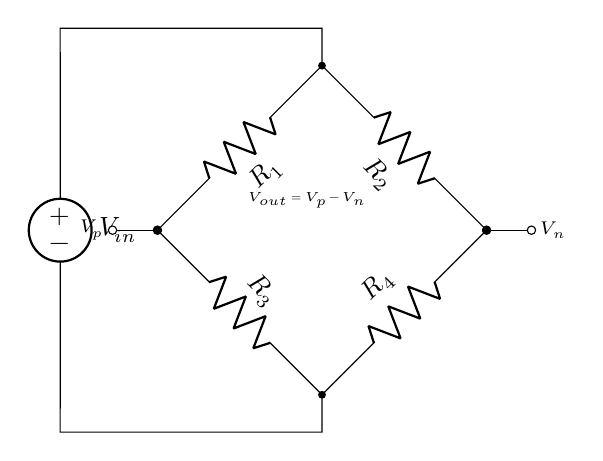
\begin{tikzpicture}[scale=0.95, transform shape]
  % Bridge nodes
  \coordinate (top) at (0, 2.2);
  \coordinate (bottom) at (0, -2.2);
  \coordinate (left) at (-2.2, 0);
  \coordinate (right) at (2.2, 0);

  % Resistors
  \draw (top) to[R, l=$R_1$] (left);
  \draw (left) to[R, l=$R_3$] (bottom);
  \draw (top) to[R, l_=$R_2$] (right);
  \draw (right) to[R, l_=$R_4$] (bottom);

  % Source
  \draw (top) -- (0, 2.7) -- (-3.5, 2.7) to[V, l=$V_{in}$] (-3.5, -2.7) -- (0, -2.7) -- (bottom);
  \fill (top) circle (1.5pt) (bottom) circle (1.5pt);
  
  % Outputs
  \draw (left) to[short, *-o] (-2.8, 0) node[left, font=\scriptsize] {$V_p$};
  \draw (right) to[short, *-o] (2.8, 0) node[right, font=\scriptsize] {$V_n$};
  
  \node[font=\tiny] at (-0.2, 0.4) {$V_{out} = V_p - V_n$};
\end{tikzpicture}
\end{tcolorbox}

For a balanced bridge with $R_1=R_2=R_3=R_4=R$, if active gauges experience strain ($\Delta R$), the output voltage is:
\begin{itemize}[leftmargin=*, itemsep=2.5pt]
  \item \textbf{Quarter Bridge (1 active gauge):} $V_{out} = V_{in} \frac{\Delta R}{4R} = \frac{GF \cdot \epsilon}{4} V_{in}$
  \item \textbf{Half Bridge (2 active gauges):} $V_{out} = V_{in} \frac{\Delta R}{2R} = \frac{GF \cdot \epsilon}{2} V_{in}$
  \item \textbf{Full Bridge (4 active gauges):} $V_{out} = V_{in} \frac{\Delta R}{R} = GF \cdot \epsilon \cdot V_{in}$ (highest sensitivity and full temperature compensation).
\end{itemize}

\subsection{5. Ultrasonic Sensors}
Ultrasonic sensors transmit high-frequency sound bursts ($\sim 40\,$kHz) and measure the echo return time to compute distance based on the \textbf{Time-of-Flight (ToF)} principle:
\begin{tcolorbox}[formulabox, title={\textbf{ToF Distance Equation}}]
\[
d = \frac{v \times t}{2}
\]
\end{tcolorbox}
where $d$ is the distance (m), $t$ is the elapsed time (s), and $v$ is the velocity of sound in the air. 
Sound velocity changes with temperature: $v \approx 331.4 + 0.607 T_C \text{ m/s}$ (where $T_C$ is the temperature in $^\circ$C). Hence, industrial level sensors include an integrated temperature sensor for real-time calibration.


% ===============================================================================
\section{Industrial Temperature and Pressure Sensors}
% ===============================================================================

\subsection{1. Resistance Temperature Detectors (RTD)}
RTDs are temperature sensors containing metallic elements whose resistance increases linearly with temperature (positive temperature coefficient).
\begin{itemize}[leftmargin=*, itemsep=2pt]
  \item \textbf{PT100:} The most common RTD, made of Platinum, having a nominal resistance of $100\,\Omega$ at $0^\circ$C, with a temperature coefficient $\alpha = 0.00385\,\Omega/\Omega/^\circ$C.
  \item \textbf{Linear Model:} For moderate temperature ranges ($0$ to $100^\circ$C):
  \[
  R(T) = R_0 (1 + \alpha T)
  \]
  \item \textbf{Self-Heating:} Since RTDs are resistive, the excitation current $I_{ex}$ creates $I_{ex}^2 R$ power dissipation, heating the element and causing a measurement error. To minimize this, $I_{ex}$ is limited to $< 1\,$mA in industrial transmitter circuits.
\end{itemize}

\subsection{2. Thermistors}
Thermistors are semiconductor-based temperature sensors that exhibit highly non-linear resistance changes.
\begin{itemize}[leftmargin=*, itemsep=2.5pt]
  \item \textbf{NTC (Negative Temperature Coefficient):} Resistance drops exponentially as temperature rises. Extremely sensitive over narrow ranges (e.g., $-50$ to $150^\circ$C).
  \item \textbf{Steinhart-Hart Equation:} The accurate non-linear model:
  \[
  \frac{1}{T} = A + B \ln R + C (\ln R)^3
  \]
  where $T$ is in Kelvin, and $A, B, C$ are curve-fitting constants.
  \item \textbf{PTC (Positive Temperature Coefficient):} Resistance increases sharply at a switching temperature. Used for overcurrent protection.
\end{itemize}

\subsection{3. Thermocouples}
A thermocouple consists of two dissimilar metal wires joined at one end (hot junction). When a temperature difference exists between the hot junction ($T_h$) and the open cold junction ($T_c$), an electromotive force (emf) is generated (Seebeck effect).
\begin{itemize}[leftmargin=*, itemsep=2.5pt]
  \item \textbf{Seebeck Voltage:}
    \[
    V_{out} = \alpha_{S} (T_h - T_c)
    \]
    where $\alpha_{S}$ is the material Seebeck coefficient ($\mu$V/$^\circ$C).
  \item \textbf{Cold Junction Compensation (CJC):} The thermocouple only measures the temperature difference $(T_h - T_c)$. To determine $T_h$, the temperature of the cold junction terminal board $T_c$ must be measured independently (using an RTD or thermistor), and the corresponding Seebeck voltage is added mathematically to the thermocouple signal.
\end{itemize}

\subsection{4. Pressure Sensors}
\begin{itemize}[leftmargin=*, itemsep=2.5pt]
  \item \textbf{Piezoelectric Pressure Sensors:} Quartz crystals generate an electrical charge $q$ when subjected to mechanical force/pressure:
    \[
    q = d \cdot F = d \cdot A \cdot P
    \]
    where $d$ is the piezoelectric charge constant, $F$ is force, $A$ is area, and $P$ is pressure. Suitable for dynamic pressure changes only (charge leaks away under static pressure).
  \item \textbf{Capacitive Pressure Sensors:} A flexible metal diaphragm acts as one plate of a capacitor. Applied pressure deforms the diaphragm, changing the plate spacing $d$, which alters the capacitance:
    \[
    C = \frac{\epsilon_0 \epsilon_r A}{d - \Delta d}
    \]
    Extremely stable and used for static industrial gauge/differential pressure transmitters.
\end{itemize}

% ===============================================================================
\section{Industrial Actuators}
% ===============================================================================

\subsection{1. DC Motors and Speed Control}
DC motors convert electrical energy to rotational torque. Speed control is achieved by varying the average armature voltage using \textbf{Pulse-Width Modulation (PWM)}.

\textbf{H-Bridge Driver:} Consists of 4 electronic switches (MOSFETs) that steer current through the armature. Toggling diagonal switch pairs allows bidirectional rotation and braking.

\subsection{2. Stepper Motors}
A stepper motor divides a full rotation into a series of equal angular increments (steps).
\begin{itemize}[leftmargin=*, itemsep=2.5pt]
  \item \textbf{Step Angle ($\theta_s$):}
    \[
    \theta_s = \frac{360^\circ}{N_s \times N_r} = \frac{360^\circ}{\text{Number of Phases} \times \text{Rotor Teeth}}
    \]
  \item \textbf{Microstepping:} By driving the stator phases with sine-cosine current profiles instead of full steps, the rotor can be positioned at intermediate angles, reducing vibration and achieving sub-degree step resolution.
\end{itemize}

\subsection{3. Servo Motors}
A servo motor is a rotary actuator that couples a standard motor (DC or AC) with a position feedback sensor (encoder) and a closed-loop controller. The controller continuously adjusts the motor drive voltage based on the error between the commanded position and the actual position.

\subsection{4. Piezoelectric Actuators}
Piezoelectric actuators use the \textbf{inverse piezoelectric effect} to produce minute displacements (nanometer scale) when an electric field is applied. Extremely high force capability but very short stroke lengths (typically $<100\,\mu$m). Used in precision micro-positioning and optical alignment.

\subsection{5. Pneumatic Actuators}
Pneumatic systems convert compressed air energy into linear or rotary motion.
\begin{itemize}[leftmargin=*, itemsep=2.5pt]
  \item \textbf{Double-Acting Cylinder:} Air is routed to one chamber to extend the piston, while exhausting air from the other. To retract the piston, the air connections are reversed.
  \item \textbf{Directional Control Valves (DCV):} A 5-port, 2-position (5/2) valve is the industrial standard for controlling double-acting cylinders.
\end{itemize}

\begin{tcolorbox}[tikzbox, title={Pneumatic Control System with a 5/2 Valve and Double-Acting Cylinder}]
\centering
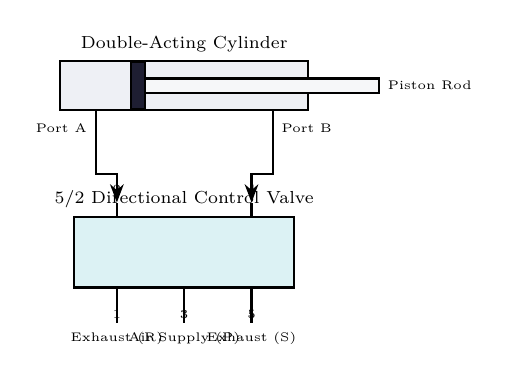
\begin{tikzpicture}[scale=0.9, transform shape]
  % Cylinder body
  \draw[thick, fill=hdrgray] (0, 0.5) rectangle (3.5, 1.2);
  \node[above, font=\scriptsize] at (1.75, 1.2) {Double-Acting Cylinder};
  
  % Piston and rod
  \draw[thick, fill=mydark] (1.0, 0.52) rectangle (1.2, 1.18);
  \draw[thick, fill=mygray] (1.2, 0.75) rectangle (4.5, 0.95);
  \node[right, font=\tiny] at (4.5, 0.85) {Piston Rod};
  
  % Ports
  \draw[thick] (0.5, 0.5) -- (0.5, 0.0);
  \draw[thick] (3.0, 0.5) -- (3.0, 0.0);
  \node[left, font=\tiny] at (0.5, 0.25) {Port A};
  \node[right, font=\tiny] at (3.0, 0.25) {Port B};

  % Valve housing
  \begin{scope}[yshift=-2.0cm]
    \draw[thick, fill=hdrteal] (0.2, 0) rectangle (3.3, 1.0);
    \node[above, font=\scriptsize] at (1.75, 1.0) {5/2 Directional Control Valve};
    
    % Ports on valve
    \draw[thick] (0.8, 1.0) -- (0.8, 1.2); \node[above, font=\tiny] at (0.8, 1.2) {2};
    \draw[thick] (2.7, 1.0) -- (2.7, 1.2); \node[above, font=\tiny] at (2.7, 1.2) {4};
    
    \draw[thick] (0.8, 0) -- (0.8, -0.2); \node[below, font=\tiny] at (0.8, -0.2) {1};
    \draw[thick] (1.75, 0) -- (1.75, -0.2); \node[below, font=\tiny] at (1.75, -0.2) {3};
    \draw[thick] (2.7, 0) -- (2.7, -0.2); \node[below, font=\tiny] at (2.7, -0.2) {5};
  \end{scope}
  
  % Connections
  \draw[thick, -Stealth] (0.5, 0) -- ++(0, -0.4) -| (0.8, -0.8);
  \draw[thick, -Stealth] (3.0, 0) -- ++(0, -0.4) -| (2.7, -0.8);
  \draw[thick] (0.8, -2.2) -- ++(0, -0.3) node[below, font=\tiny] {Exhaust (R)};
  \draw[thick] (2.7, -2.2) -- ++(0, -0.3) node[below, font=\tiny] {Exhaust (S)};
  \draw[thick] (1.75, -2.2) -- ++(0, -0.3) node[below, font=\tiny] {Air Supply (P)};
\end{tikzpicture}
\end{tcolorbox}

\newpage

% ===============================================================================
% QUICK REVISION PAGE
% ===============================================================================
\begin{center}
  {\large\bfseries\color{myred} Quick Revision --- Module 1}\\[3pt]
  {\small\color{mydark} Sensors \& Actuators $|$ PE-EC802B}
\end{center}
\noindent{\color{myred}\rule{\linewidth}{1.2pt}}
\vspace{4pt}

\begin{tcolorbox}[formulabox, title={\textbf{Key Formulas at a Glance}}]
\renewcommand{\arraystretch}{1.35}
\begin{tabularx}{\linewidth}{B{5.2cm} X}
Potentiometer Loading Error & $V_{out} = V_{in} \frac{x}{1 + x(1-x)\frac{R_p}{R_L}}$ \\[4pt]
Gauge Factor & $GF = \frac{\Delta R / R}{\epsilon} = 1 + 2\nu + \frac{\Delta\rho/\rho}{\epsilon}$ \\[4pt]
RTD Resistance & $R(T) = R_0 (1 + \alpha T)$ \\[4pt]
Steinhart-Hart (Thermistor) & $\frac{1}{T} = A + B \ln R + C (\ln R)^3$ \\[4pt]
Ultrasonic Distance & $d = \frac{v \times t}{2}$ where $v \approx 331.4 + 0.6 T_C$ \\[4pt]
Stepper Step Angle & $\theta_s = \frac{360^\circ}{N_s \times N_r}$ \\
\end{tabularx}
\end{tcolorbox}

\begin{tcolorbox}[defbox, title={\textbf{One-Line Definitions}}]
\begin{itemize}[leftmargin=*, itemsep=2pt, topsep=0pt]
  \item \textbf{LVDT:} A transformer-based passive sensor that outputs an AC voltage proportional to the linear displacement of a sliding core.
  \item \textbf{Gauge Factor:} The ratio of fractional change in resistance to the mechanical strain applied to a strain gauge.
  \item \textbf{Poisson's Ratio ($\nu$):} The ratio of lateral transverse strain to longitudinal axial strain.
  \item \textbf{PT100:} A platinum RTD having $100\,\Omega$ resistance at $0^\circ$C and a standard positive temperature coefficient.
  \item \textbf{Seebeck Effect:} The generation of a voltage at the open terminals of two dissimilar metals due to a temperature difference.
  \item \textbf{Microstepping:} Controlling stepper phases with fractional currents to position the rotor between full steps.
\end{itemize}
\end{tcolorbox}

\begin{tcolorbox}[tikzbox, title={\textbf{Sensor \& Actuator Technology Comparisons}}]
\centering
\par\noindent
\renewcommand{\arraystretch}{1.3}
\begin{tabularx}{\linewidth}{|B{2.8cm}|Y|Y|Y|}
\hline
\textbf{Property} & \textbf{RTD} & \textbf{Thermocouple} & \textbf{Thermistor} \\ \hline
\textbf{Linearity} & Highly Linear & Non-linear & Exponentially Non-linear \\ \hline
\textbf{Temp.~Range} & Wide ($-200$ to $850^\circ$C) & Extremely Wide ($-270$ to $1800^\circ$C) & Narrow ($-50$ to $150^\circ$C) \\ \hline
\textbf{Sensitivity} & Moderate & Low ($\mu$V/$^\circ$C) & Very High ($\Omega$/$^\circ$C) \\ \hline
\textbf{CJC Required} & No & Yes & No \\ \hline
\end{tabularx}

\vspace{0.3cm}
\begin{tabularx}{\linewidth}{|B{2.8cm}|Y|Y|}
\hline
\textbf{Property} & \textbf{Stepper Motor} & \textbf{Servo Motor} \\ \hline
\textbf{Control Mode} & Open-loop (no sensor feedback) & Closed-loop (requires encoder) \\ \hline
\textbf{Torque at Speed} & High at low speed; falls at high speed & Constant torque throughout speed range \\ \hline
\textbf{Precision} & Limited by step angle/microstepping & High (limited only by encoder resolution) \\ \hline
\textbf{Cost \& Complexity} & Low cost; simple drive interface & High cost; complex servo tuning \\ \hline
\end{tabularx}
\end{tcolorbox}

\begin{tcolorbox}[exambox, title={\textbf{Frequently Asked / Viva Questions}}]
\begin{enumerate}[leftmargin=*, itemsep=4pt]
  \item \Q{Why are LVDT secondary windings connected in series opposition?}
    This connection ensures that the induced voltages in the two secondaries ($V_{s1}$ and $V_{s2}$) subtract. When the core is centered, the voltages cancel, producing $V_{out}=0$. This establishes a clear zero reference point (null position) to identify direction and magnitude.
  \item \Q{Explain the role of dummy strain gauges in bridge circuits.}
    Dummy strain gauges are exposed to the same temperature as the active gauge but are not subjected to mechanical strain. By placing them in adjacent bridge arms, temperature-induced resistance changes cancel out, preventing thermal drift errors.
  \item \Q{What is the Seebeck effect, and how is it used in thermocouples?}
    It states that when two junctions of dissimilar metals are at different temperatures, an electrical potential difference (voltage) is generated. Thermocouples use this to measure the temperature difference between the hot and cold junctions.
  \item \Q{Why is 4-wire measurement preferred for RTDs in industrial settings?}
    In 2-wire RTDs, the resistance of the lead wires adds to the measurement, causing a positive temperature error. In 4-wire RTDs, two wires supply a constant current while the other two high-impedance wires measure the voltage across the sensor element, completely eliminating lead resistance error.
  \item \Q{Explain the physical reason behind NTC behavior in thermistors.}
    As temperature increases in a semiconductor material, thermal energy excites more valence electrons into the conduction band. This increases the concentration of free charge carriers, leading to a drop in electrical resistance.
  \item \Q{Compare Full-step, Half-step, and Microstepping in stepper motor control.}
    Full-step drives one or two phases fully, moving the rotor by its full step angle. Half-step toggles between one and two phases, cutting step angle in half. Microstepping applies sine-cosine current profiles to stator coils, positioning the rotor smoothly at intermediate microsteps, reducing vibration.
\end{enumerate}
\end{tcolorbox}

\end{document}
